\documentclass[pdftex,letterpaper,twocolumn,10pt]{sig-alternate-10pt}
%\documentclass[pdftex,letterpaper]{sig-alternate}

\newcommand{\subparagraph}{}
%\documentclass[pdftex,letterpaper]{article}
\newcommand{\AUTHORS}{Victor Costan, Tiffany Yu-Han Chen, Ravi Netravali}
%\newcommand{\TITLE}{Super-Rational Congestion Control}
\newcommand{\TITLE}{\name{} - Network Performance Measurements} 
\newcommand{\KEYWORDS}{}
\newcommand{\CONFERENCE}{}
\newcommand{\PAGENUMBERS}{yes}       % "yes" or "no"
%\newcommand{\TOAPPEAR}{no}
%\newcommand{\comment}[1]{}
\usepackage{ifthen}
\usepackage{endnotes}

\ifthenelse{\equal{\PAGENUMBERS}{yes}}{%
\usepackage[nohead,
            left=4.5pc,right=4.5pc,top=4.5pc,
            footskip=0.5in,bottom=6pc,
            columnsep=2pc
            ]{geometry}
}{
\usepackage[noheadfoot,
            left=4.5pc,right=4.5pc,top=4.5pc,
            footskip=0.5in,bottom=6pc,
            columnsep=2pc
	    ]{geometry}
}

\usepackage{fancyhdr}
%\usepackage[numbers]{natbib}
\usepackage{booktabs}
\renewcommand{\toprule}{}
\renewcommand{\bottomrule}{}
\usepackage[compact]{titlesec}

\usepackage{color}
\usepackage{mathptmx}   % Times + Times-like math symbols
\usepackage{courier}
\usepackage[scaled=0.92]{helvet}
\usepackage{xspace}

\usepackage{color}
\usepackage{colortbl}
\usepackage{graphicx}
\usepackage{import}
\usepackage{amsmath}
\usepackage{amssymb}
\usepackage{algorithm}
\usepackage{url}
\usepackage{ifthen}
\usepackage{color}
%\usepackage{endnotes}
%\usepackage{graphicx}
\usepackage{listings}

%\usepackage{clrscode}
%\usepackage[noeka]{mathrmletter}
\usepackage[loose]{subfigure}
%\usepackage{caption}
%\usepackage{subcaption}
\usepackage{multirow}
\usepackage[noend]{algorithmic}
\usepackage{html, makeidx}

%\usepackage{thumbpdf}
%%\ifthenelse{\isundefined{\wantBW}}{%
%%  \usepackage[colorlinks]{hyperref}%        % for online version
%%}{%
  \usepackage[pdfborder={0 0 0}]{hyperref}% % for paper (B&W) version
%%}
\newcommand{\URL}[1]{\url{#1}}

\interfootnotelinepenalty=10000  % Split footnote are annoying


%%%%% Setup for PDF
% \hypersetup{%
% pdfauthor = {\AUTHORS},
% pdftitle = {\TITLE},
% pdfsubject = {\CONFERENCE},
% pdfkeywords = {\KEYWORDS},
% bookmarksopen = {true}
% }

%\setlength{\parindent}{0pt}
%\setlength{\parskip}{\baselineskip}
\renewcommand{\headrulewidth}{0pt}

\ifthenelse{\equal{\PAGENUMBERS}{yes}}{%
  \pagestyle{plain}
}{%
  \pagestyle{empty}
}

%\usepackage[font=bf]{caption}
\usepackage{comment}

% following two lines were remarked in hotnets version
% \clubpenalty=1000  % Don't allow orphans
% \widowpenalty=1000 % Don't allow widows

%\newcommand{\affaddr}{\fontsize{12}{14}\selectfont}
%\newfont{\ttlfnt}{phvb8t at 18pt}
%\newfont{\aufnt}{phvr8t at 12pt}
%\newfont{\affaddr}{phvr8t at 10pt}
%\newfont{\bibfnt}{ptmr8t at 10pt}
%\title{\ttlfnt\TITLE}
%{\affaddr Massachusetts Institute of Technology}}
\date{}

%%%%%%%%%%%% Macros by me %%%%%%%%%%%%%%%
\newcommand{\ea}{et al.}
\newcommand{\ie}{i.e.}
\newcommand{\eg}{e.g.}

\newcommand{\name}{NetMap}

\newcommand{\ith}{$i^\text{th}$}
\newcommand{\tth}{$t^\text{th}$}
\newcommand{\lth}{$\ell^\text{th}$}
\newcommand{\gth}{$g^\text{th}$}

\newcommand{\para}[1]{\medskip\noindent{\bf #1}}

% peanut gallery comments; from Mike Walfish
%
%
% NOTE: Comment out the line below if you want a draft with no red comments.
% NOTE: Commenting out this line may replace some of the red comments with
%       extra spaces or newlines.
\def\noeditingmarks{}
%
\newcommand{\textred}[1]{\textcolor{red}{#1}}
\ifx\noeditingmarks\undefined
   \newcommand{\pgwrapper}[2]{\textred{#1: #2}}
\else
   \newcommand{\pgwrapper}[2]{}
\fi
\newcommand{\hb}[1]{\pgwrapper{HB}{#1}}
\newcommand{\as}[1]{\pgwrapper{YC}{#1}}
\newcommand{\yc}[1]{\pgwrapper{AS}{#1}}
\newcommand{\ls}[1]{\pgwrapper{LS}{#1}}
% end peanut gallery comments

%margins
\setlength{\columnsep}{.33in}
\setlength{\textheight}{9.25in}
\setlength{\textwidth}{7in}

%\usepackage{microtype}

\usepackage{textcomp}

\newcommand{\Prob}{{\mathbb P}}

%% ACM Copyright Block
%
%% \usepackage{float}
%% \floatstyle{plain}
%% \newfloat{acmcr}{b}{acmcr}
%% \newcommand{\acmcopyright}{%
%% \begin{acmcr}
%% \parbox[b]{\columnwidth}{%
%% \vspace{0.2in}
%% \small
%% Permission to make digital or hard copies of all or part of this work
%% for personal or classroom use is granted without fee provided that
%% copies are not made or distributed for profit or commercial advantage
%% and that copies bear this notice and the full citation on the first
%% page.  To copy otherwise, to republish, to post on servers or to
%% redistribute to lists, requires prior specific permission and/or a fee.

%% \emph{SIGCOMM'09}, August XX--XX, 2009, ...............\\
%% Copyright 2009 ACM 978-1-60558-175-0/08/08 \dots \$5.00.}
%% \end{acmcr}}

%%%%%%%%%%%%%%%%%%%%%%%%  START DOCUMENT  %%%%%%%%%%%%%%%%%%%%%%%%%%%

\makeatletter

\global\def\section{\@startsection {section}{1}{\z@}%
                                   {-1.5ex \@plus -0.8ex \@minus -.1ex}%
                                   {0.6ex \@plus.2ex}% changed this
                                   {\normalfont\bfseries\scshape\fontsize{11}{13}\selectfont}}
\global\def\subsection{\@startsection{subsection}{2}{\z@}%
                                     {-1.25ex\@plus -0.8ex \@minus -.1ex}%
                                     {0.3ex \@plus .1ex}% changed this
                                     {\normalfont\bfseries\fontsize{10}{12}\selectfont}}
\global\def\subsubsection{\@startsection{subsubsection}{3}{\z@}%
                                     {-1ex\@plus -1ex \@minus -.1ex}%
                                     {0.1ex \@plus .1ex}% changed this
                                     {\normalfont\itshape\fontsize{10}{12}\selectfont}}

% following were commented out for hotnets version:
%\global\def\@maketitle{%
%  \newpage
%  \null
%  \vskip -0.31in%
%  \null
%  \begin{center}%
%  \let \footnote \thanks
%    {\LARGE \@title \par}%
%    \vskip 0.75em%
%    {\large
%      \lineskip .5em%
%      \begin{tabular}[t]{c}%
%        \@author
%      \end{tabular}\par}%
%    \vskip 1em%
%    {\large \@date}%
%  \end{center}%
%  \par
%  \vskip 0.5em}

%\def\newblock{\hskip .11em plus .33em minus .07em}

\clubpenalty=10000
\widowpenalty = 10000

\begin{document}
\conferenceinfo{SIGCOMM'13,} {August 13--17, 2013, Taipei,
Taiwan.}
\CopyrightYear{2012}
\crdata{978-1-4503-1419-0/12/08}
\clubpenalty=10000
\widowpenalty = 10000

%\conferenceinfo{SIGCOMM'11,} {... 2011, Toronto, Canada}
%\CopyrightYear{2011}
%\crdata{978-1-60558-594-9/09/08}

 % \setlength{\paperwidth}{8.5truein}
 % \setlength{\paperheight}{11.0truein}
 % \setlength{\pdfpagewidth}{\paperwidth}
 % \setlength{\pdfpageheight}{\paperheight}

\title{\TITLE}
%\author{\AUTHORS}
%\if 0
%\numberofauthors{3}
\author{\alignauthor Victor Costan, Tiffany Yu-Han Chen, Ravi Netravali\\
\affaddr{Computer Science and Artificial Intelligence Laboratory}\\
\affaddr{Massachusetts Institute of Technology, Cambridge, Mass., USA} \\
\email{\{costan,yuhan,ravinet\}@mit.edu}\\}
%(January 27, 2013: In double-blind submission for review)}
%\fi
%\date{January 27, 2012 (In double-blind submission for review)}

\maketitle

\begin{sloppypar}

\begin{abstract}
\label{s:abstract}

We introduce a platform for measuring wireless Internet access performance
across the world's cellular and WiFi networks. Our platform consists of a
library for collecting network performance measurements on Android devices, a
pipeline for storing and processing the performance measurements, and tools and
sample code for accelerating the development of location-based mobile games
that contribute peformance measurements to our project. We plan to develop one
such game, and release it for free on the Android market. Players pay for the
by game by implicitly allowing us to use their phone to measure network
performance. We also opened up and documented our platform, hoping to influence
other (more talented) game developers to build games on top of our platform.


\end{abstract}

\ifthenelse{\isundefined{\onlyAbstract}}{%

\section{Introduction}
\label{s:intro}


Recent years have seen an immense growth in the number of wireless devices in use. The functionality of these devices has similarly evolved as one can find a mobile application for just about any task. In turn, the need for efficient and widespread wireless network coverage is at a high. However, today, customers often experience poor network coverage over both WiFi and cellular networks. Application developers find it difficult to understand how to optimize their application's performance for different devices over wireless networks. Researchers struggle to find data to test proposed improvements in wireless network and device performance. This arises from a lack of information about the behavior and performance of wireless networks for different devices, locations, and times. 

This work describes the design, implementation, and experimental evaluation of NetMap, a system that provides a battery-aware network performance measurement collection service with a simple API for mobile devices. Our main contributions are a measurement collection API designed for games as well as a packaging mechanism to collect performance data in a mobile device game. 

Our API provides a means to collect various types of data including user-specific data such as device model and location (GPS), network performance data including latency, bandwidth, and average round-trip-time, and neighboring network infrastructure information such as neighboring network type and signal strength to neighboring towers/access points. It is specifically designed for mobile device games. Game development is straightforward, as designers are not required to know how our measurements are collected, processed, stored, etc. Game designers simply use functions in our API to collect the requested data.

We developed a scheme which aligns incentives so game players collect measurements while playing. That is, we tie measurement collection at real-world locations with movement and actions in the mobile games. Ideally, the provided measurement library would be called upon when a game player moves (reflecting movement in real-life and consequently movement in-game). Measurement collection can thus be widespread as users provide measurements from various locations while playing their mobile device game.

Users of these mobile games are aware that they will be collecting information on network connectivity that will be used for research purposes. However, beyond providing permission, gameplay is the user's sole focus, as no additional effort must be expended to gather, store, or analyze the network performance measurements. We are also battery-aware so battery-intensive data collection and transfers are done only when battery permits reducing user overhead. 

Targeted results of using NetMap and a mobile device game are a collection of various network performance statistics such as bandwidth, latency, average round-trip-time, etc., user statistics such as phone models and battery, and a comprehensive map of how different wireless networks behave across various regions. From these results, researchers and game developers can infer cellular network and WiFi performance for different areas, devices, and times. Additionally, this will provide a reliable and up-to-date source of data for researchers to use in developing improvements for wireless and mobile device connectivity. 



\section{Related Work}
\label{s:related}


Network Diagnostic Tool (NDT)~\cite{NDT} collects performance data over wireless links using a client/server architecture. The server consists of a webserver and an analysis engine. The client communicates with this enhanced server to perform diagnostic tests including web page request and the server collects the resulting measurements and attempts to identify the cause of performance issues. The primary goal of ndt is to identify network performance issues, which occur close to users (eg. incorrectly set TCP buffers). The server locations are all known (clients connect to one of the closest servers) and servers collect data making it easier to measure certain statistics such as one-way latency.


Dasu~\cite{dasu-sanchez} is a measurement platform for the Internet's edge. Dasu can support broadband characterization as well as internet measurement experiements. They design Dasu for the edge of the Internet so measurements reflect end users' views of the services they are using. Dasu also does not use dedicated infrastructures for experimentation. Instead, they use an incentive model to make sure it is widely adopted at the edge of the Internet. Dasu has a distributed set of clients and a set of management services. Clients perform measurements and the management services configure clients,  perform administration of experiments, and handle data collection. Dasu provides a programming interface that is flexible to run many kinds of tests (when-then model where condition dictates type of test). 

MIST~\cite{wittie:mist}, a distributed platform for measuring cellular network performance of users with hopes of aiding mobile application developers. MIST is a mobile app connected to server back-end. Communication between the mobile application on the user's device and the servers are performed to measure characeteristics of the cellular networks, including latency, jitter, throughput, etc. The database at the server saves the measurement data along with mobile device info/configuration from the test. Perk is that MIST can be deployed on top of mobile devices (don't have to change cell network infrastructure). App first collects info about mobile device, service provider, and test location. Mobile app connects to closest server to get most accurate measurements. Then app sends packets of set byte-size to analyze uplink and downlink latency, throughput, and timeouts. Difference from ours is that MIST is an app designed to get such measurements for mobile app developers (we wrap measurement collection in a game so it is not specifically used for this purpose). 

Balachandran et al.~\cite{Balachandran-sigmetrics} capture a workload at a large conference and analyze it to understand user behavior and network performance. They collect a continuous trace of SNMP data from all APs in the conference main room as well as a tcpdump trace of network-level headers of packets going through switch which all APs connected to. This provided aggregate packet level statistics of all traffic passing through these APs at the link, network and transport layers. Also, they obtained information about the users associated with the APs such as their MAC addresses, SNR, and effective throughput. They inferred the number of distinct wireless users by counting the number of distinct MAC addresses in packets passing through the APs present. The primary goal was to analyze user behavior in terms of mobility, application popularity, data rates, etc. In terms of network performance, they measure the aggregate offered load for each of the APs and observe the bursty behavior. They also measure packet errors by using the SNMP trace where APs count the total number of packets transmitted and received, and the number of packets in error (account for inbound packets that could not be delivered to higher layer and outbound packets that cant be transmitted due to channel). 

VISUM~\cite{VISUM} is a framework for wireless network monitoring that uses set of agents within network (scales better than centralized) to monitor network devices and store info at repositories. VISUM also visualizes the data into real-time statistical graphs and interactive network topology maps. They target single-hop wireless networks.  Thus, VISUM relies on a distributed architecture (agents at different locations) to monitor large scale wireless networks. Agents collect measurement info from network devices using SNMP and store the data in a centralized repository (data stored per device using device OID).  

\section{Design Overview}
\label{s:overview}

\subsection{The Network Performance Measurement Library}
We measure more than 200 types of network data, including device-specific data such as device model, 
location data, network performance data including latency, bandwidth, and average round-trip-time, 
neighboring network infrastructure information such as neighboring network type and signal strength to 
neighboring towers/access points, and the DHCP information. All the data is stored in JSON format, so
that researchers can easily parse it.


{\bfseries Device-Specific Information.} \name{} collects device-specific information including the device ID 
(IMEI or ESN), the device type (GSM or CDMA), the software version. With the device ID, we can 
identify a device, track the device, and discard bad data that comes due to cheating. We can 
even provide personalized network usage diaries which allow users to better understand their network 
using habits.
Collecting OS version allows us to infer the effect of system and harware on the network performance. \name{} also 
logs SIM card information, such as the phone number, the SIM card operator (AT\&T, T-Mobile, etc.),
the radio type (EDGE, GPRS, HSDPA, etc.).
This permits us to create the map of network quality for each phone carrier or type, and to track how the network quality 
evolves over time.

{\bfseries Location.} The system gathers the user's location information from the GPS or network location provider. 
For the GPS, in addition to the latitude and longitude, our system also collects information 
about the observed satellites, including the almanac, ephemeris, azimuth, elevation, and SNR.
We plan to use the stallites information to detect users that cheat the game by faking their GPS locations.
Because GPS is unavailable indoors, we also use the network location provider's locations.
%gather location estimation from the network provider
%and verify its eligibility with the cell tower/AP information we collect.


{\bfseries Network Infrastructure Information.} \name{} collects information about
neighboring WiFi APs and cell towers. The cell tower information includes the mobile country code (MCC), 
mobile network code (MNC), location area code (LAC), and the signal strength; the WiFi AP information
includes the MAC address, SSID, IP address, frequency band, RSSI, link speed, etc.
With the locations where users observed the cell tower/AP, we can approximate the location of 
each cell tower/AP. Many research projects~\cite{ctrack, vtrack-sensys09} have focused on using 
energy efficient sensors to provide accurate position estimation, but most of them suffer from scalability
problem due to lack of cell tower/AP observations. We belive we can greatly assist those projects
with the crowd-sourced data that we have. However, neighboring GSM cell tower information isn't 
universally available across all phones. Some phone models limit the cell information to only 
the connected tower or do not make it available at all.

\name{} also collects the DHCP information, including the assigned IP, network mask, IP of the DHCP server, etc.
DHCP information is useful for inferring the network topology, and for cheating detection.
 
 
{\bfseries Network Performance.} We collect sophisticated network performance measurements 
such as the network latency, bandwidth, average round-trip-time, and some TCP variables. 
For researchers, they can use the information for research on improving network reliability and performance or
 making tradeoffs when designing systems. 
For normal users, these measurements help them choose the network carrier and device which provide
 the best reception in their neighborhood. 

We use the Network Diagnostic Tool (NDT)~\cite{NDT} to collect network information. NDT measures various network 
performance metrics between the mobile device and their distributed servers. There are some straightforward 
and incredibly tedious problems in measuring the network performance. First, in order to get individual latency
measurements for both the uplink and downlink, one needs to consider the time 
synchronization problem between the device and the server. Second, to eliminate the noise in the measurement, 
one needs to maintain servers in multiple places. 
NDT solves the time synchronization problem, and it maintains 81 servers in 27 coutries. This allows \name{}
to provide accuracy network performance measurements across the world.

\subsection{Battery/Network Awareness}
There are two important aspects that designers need to take into account when implementing a mobile 
programming API. First, the API should be energy-efficient. 
Games using the API should avoid caonsuming the users ; second, the API should
not drain the user's data plan or make the user pay extra money. 
 
\name{} addresses these two problems by incorporating the concept of battery and network aware. 
To be battery aware, \name{} monitors the battery level and status. Games using the API would get
notified when the phone is charging or when the battery level is low, and take certain actions
to save energy. For example, if the phone is charging, the game can start uploading the measurements 
it collected to the server or taking measurements more frequently. 

\name{} is also network aware. \name{} monitors the network type that the device is currently using, 
and notifies the games that using the API if the user switches to either WiFi or cellular network.
Games can react to the notification by uploading all the collected measurements to the server when
the phone is using WiFi.


\subsection{Preliminary Results}
\label{ss:results}

\begin{figure}[t]
  \center{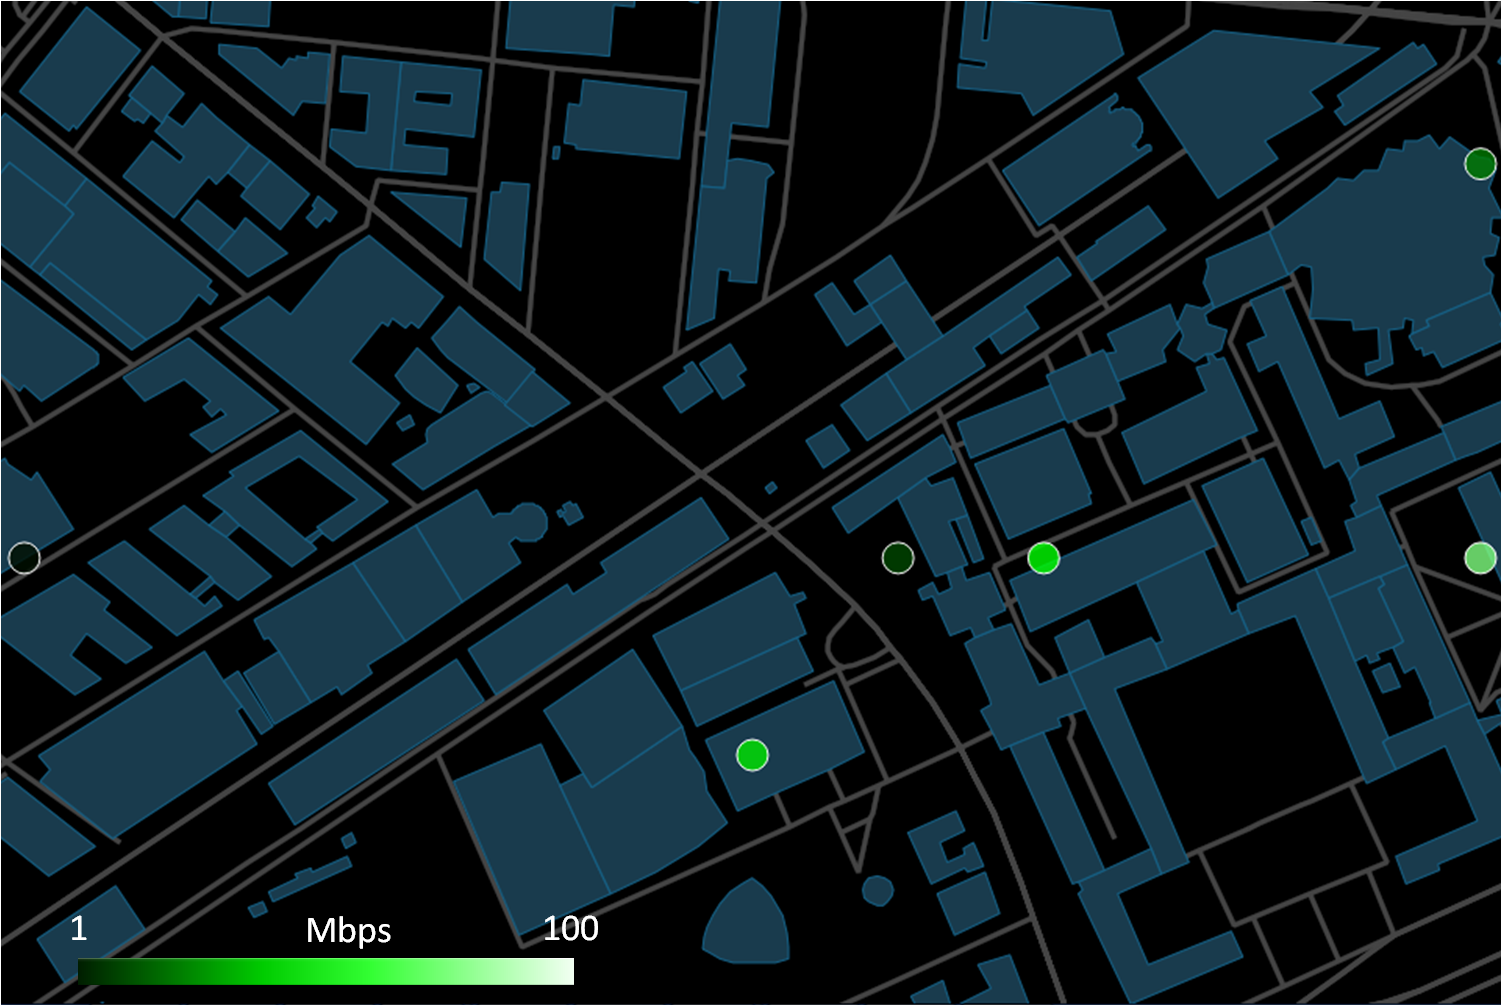
\includegraphics[width=85mm]{figures/bw.png}}
  \caption{
    The map of the WiFi/cellular network bandwidth.
  }
  \label{fig:bw}
\end{figure}

\begin{figure}[t]
  \center{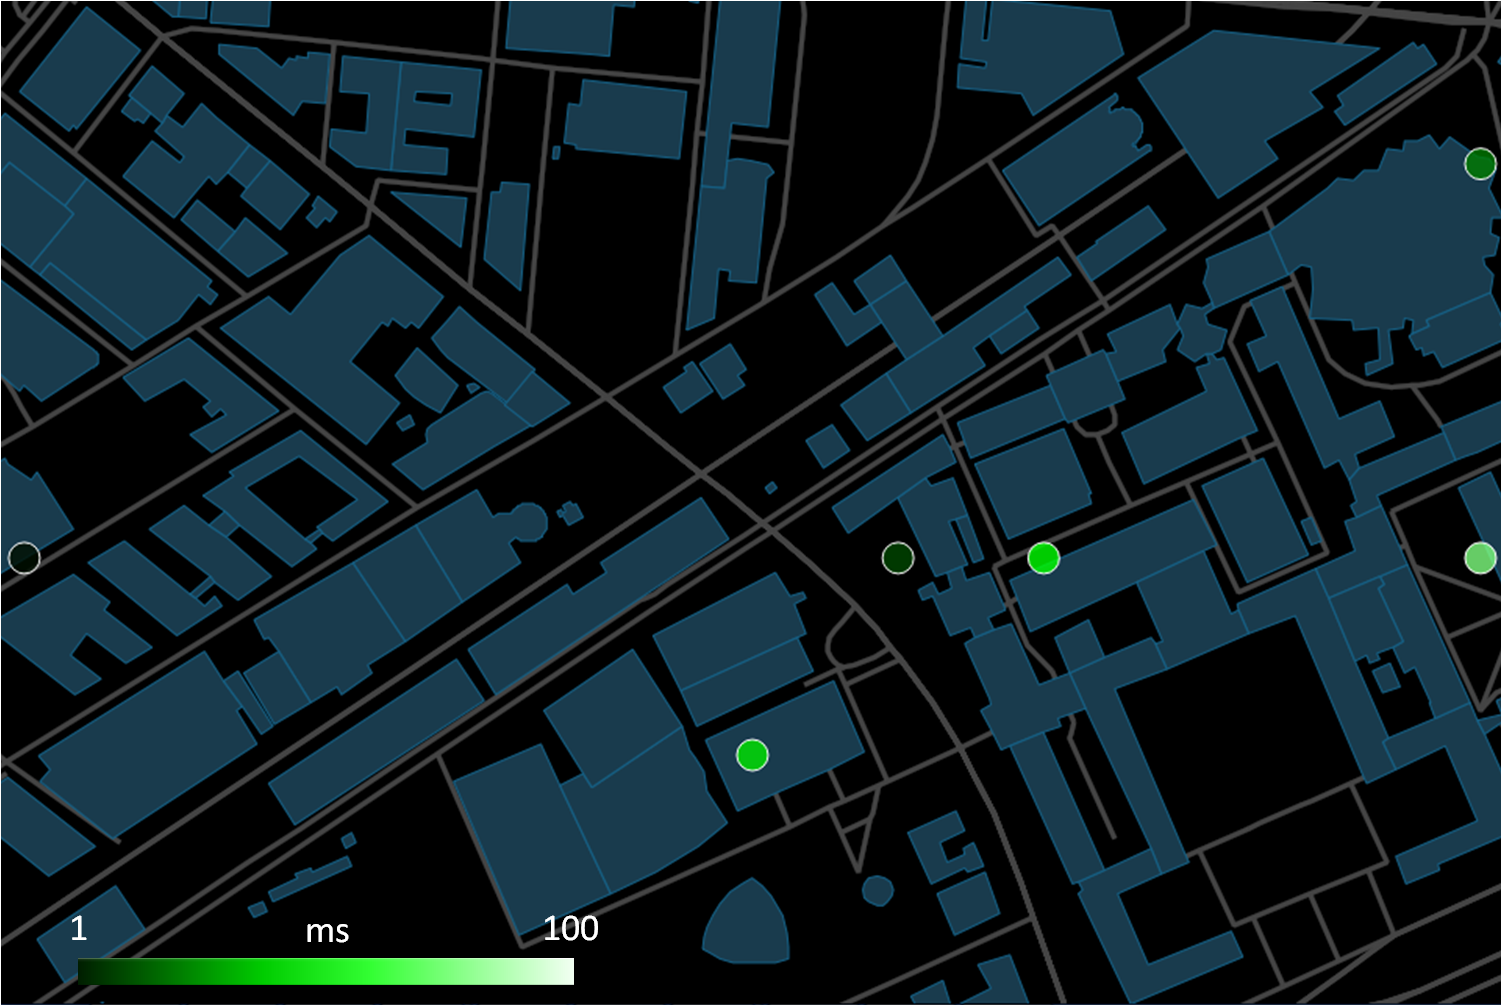
\includegraphics[width=85mm]{figures/rtt.png}}
  \caption{
    The map of the WiFi/cellular network average round-trip-time.
  }
  \label{fig:rtt}
\end{figure}

In this section, we present the map of several network performance
metrics based on the data we collected. This is one of the many possible 
applications that can be realized using \name{}'s data. 

We implemented an Android application using \name{}'s measurement 
library API and collected data around the MIT campus. 
All the measurements are uploaded and stored in the \name{} Server.
To visualize the network performance metrics on a map, we divide the map
into multiple grids, average all the values within a particular grid, and
plot the average value as a circle at the center of the grid. 

{\bfseries Bandwidth.}
Figure~\ref{fig:bw} shows the map of the WiFi/cellular network bandwidth.
As we mentioned in the introduction, wireless Internet connection performance 
varies greatly. The map clearly illustrates the spatial variation. The bandwidth
ranges from 1 to 90 Mbps within a small distance, and under the same administrative
domain (MIT's IS\&T). Therefore, a possible consequence is that we'll need to 
be able to handle hi-resolution data to produce an accurate map.

{\bfseries Average Round-Trip-Time.}
Figure~\ref{fig:rtt} presents the map of the WiFi/cellular network average
round-trip-time. We make two observations. First, the average RTT also 
varies with location (from 20 to 800 ms). Second, there is no clear 
correlation between the network bandwidth and the average RTT. The place with a
higher bandwidth does imply a shorter RTT. 

\section{Conclusion}
\label{ss:conclusion}
In this paper, we present \name{}, a system that
provides a battery-aware network performance
measurement collection service with a simple API for
mobile devices. \name{} is easy to integrate, unobstrusive,
cheat-proof, and data-hungry. The measurement library
collects more than 200 types of network metrics and is
both battery and network aware. Preliminary results
have demonstrated that it is possible to assist both
researchers and normal users to better understand the
network performance with \name{}'s data.

%\begin{flushleft}
%\setlength{\bibsep}{1pt}
%\bibsep=1pt
\bibliographystyle{abbrv}
\bibliography{ref-hacked}
%\bibliography{ref,rfc}
%\end{flushleft}
}

\section{Appendix}
\label{s:appendix}

\subsection{An Example of the Measurement}
\tiny
\begin{verbatim}
{
    "serial": 87,
    "app_id": 1071359345,
    "app_uid": "4842233025919687312",
    "created_at": "2013-05-14T00:41:44.993Z",
    "ip": "18.111.84.182",
    "data": {
        "uid": "1071359345.4842233025919687312.puumX9DcBa6UbfTfBdI6g4fSKew_h_FUh7gEgzrUGBM",
        "timestamp": 1368492034049,
        "location": {
            "latitude": 42.3587538,
            "longitude": -71.0949983,
            "provider": "network",
            "timestamp": 1368491627298,
            "accuracy": 31.571
        },
        "battery": {
            "status": "discharging",
            "plugged": "unknown",
            "charge": {
                "level": 91,
                "scale": 100
            },
            "health": "unknown"
        },
        "cellular": {
            "phoneId": "353918055485722",
            "line1Number": "16172309694",
            "networkOperator": "310260",
            "networkOperatorName": "T-Mobile",
            "simOperator": "310260",
            "simOperatorName": "",
            "softwareVersion": "03",
            "networkCountryISO": "us",
            "simCountryIso": "us",
            "simSerialNumber": "8901260562590079971",
            "isRoaming": false,
            "callState": 0,
            "subscriberId": "310260569007997",
            "phoneType": "gsm",
            "radioType": "edge",
            "dataActivity": "none",
            "dataState": "disconnected",
            "simState": "ready"
        },
        "gps": {
            "enabled": true,
            "started": true,
            "timeToFix": 0,
            "satellites": [
                {
                    "prn": 1,
                    "used": false,
                    "almanac": true,
                    "ephemeris": true,
                    "azimuth": 104,
                    "elevation": 67,
                    "snr": 0
                },
                { ... },
                {
                    "prn": 88,
                    "used": false,
                    "almanac": false,
                    "ephemeris": false,
                    "azimuth": 254,
                    "elevation": 34,
                    "snr": 0
                }
            ]
        },
        "wifi": {
            "enabled": true,
            "connection": {
                "ssid": "\"MIT\"",
                "hidden": false,
                "bssid": "00:21:d8:49:a3:8d",
                "mac": "10:68:3f:45:82:2b",
                "rssi": "-68",
                "linkMbps": 39,
                "state": "COMPLETED",
                "ip": "18.111.84.182"
            },
            "dhcp": {
                "ip": "18.111.84.182",
                "netmask": "255.255.224.0",
                "gateway": "18.111.64.1",
                "dhcpServer": "18.7.50.68",
                "dns1": "18.71.0.151",
                "dns2": "18.70.0.160",
                "lease": 86400
            },
            "aps": [
                {
                    "ssid": "MIT",
                    "bssid": "00:21:d8:49:a3:8d",
                    "channelMhz": 5805,
                    "signalDb": -57,
                    "timestamp": 1368492027217,
                    "capabilities": "[ESS]"
                },
                { ... },
                {
                    "ssid": "MIT N",
                    "bssid": "00:21:d8:49:c3:bf",
                    "channelMhz": 5805,
                    "signalDb": -85,
                    "timestamp": 1368492027217,
                    "capabilities": "[ESS]"
                }
            ]
        },
        "gsm": {
            "enabled": true,
            "type": 2,
            "cid": 60493,
            "lac": 5103,
            "rssi": 8,
            "ber": 0,
            "numOfCells": 1,
            "cells": [
                {
                    "type": 2,
                    "cid": 60491,
                    "lac": 5103,
                    "rssi": 2,
                    "psc": -1
                }
            ]
        },
        "ndt": {
            "provider": "wifi",
            "cwndtime": "0.9020",
            "PktsIn": "9399",
            "SmoothedRTT": "18",
            "AckPktsOut": "0",
            "AckPktsIn": "9399",
            "bw": "17.77",
            "congestion": "0",
            "c2sData": "6",
            "SubsequentTimeouts": "0",
            "CurCwnd": "52128",
            "DataBytesIn": "0",
            "cwin": "0.5192",
            "WinScaleSent": "7",
            "SndLimTimeRwin": "870708",
            "StartTimeUsec": "789481",
            "s2cData": "8",
            "MinRTT": "9",
            "CurRTO": "218",
            "MaxMSS": "1448",
            "spd": "18.09",
            "bad_cable": "0",
            "rwin": "0.5083",
            "aspd": "0.00000",
            "SndLimBytesRwin": "2379840",
            "rttsec": "0.018214",
            "MinRTO": "210",
            "Timeouts": "1",
            "timesec": "10.00",
            "MaxRwinSent": "5888",
            "SlowStart": "247",
            "PktsRetrans": "72",
            "WinScaleRcvd": "5",
            "SndWinScale": "5",
            "s2cAck": "7",
            "RcvWinScale": "7",
            "NagleEnabled": "1",
            "DSACKDups": "18",
            "minCWNDpeak": "2896",
            "DupAcksIn": "589",
            "MinRwinSent": "5792",
            "MaxSsthresh": "94894680",
            "MinRwinRcvd": "14624",
            "DataPktsIn": "0",
            "half_duplex": "0",
            "CWNDpeaks": "20",
            "DataPktsOut": "15458",
            "SampleRTT": "20",
            "maxCWNDpeak": "68056",
            "waitsec": "0.22",
            "loss": "0.001164446",
            "DupAcksOut": "0",
            "SndLimTransCwnd": "50",
            "FastRetran": "17",
            "link": "0",
            "X_Sndbuf": "176344",
            "SndLimBytesCwnd": "20366280",
            "ECNEnabled": "0",
            "BytesRetrans": "104256",
            "PktsOut": "15458",
            "OtherReductions": "132",
            "CWND-Limited": "907.95",
            "CongestionOverCount": "141",
            "MaxRTO": "264",
            "rwintime": "0.0861",
            "order": "0.0627",
            "SndLimTimeSender": "120444",
            "MaxRTT": "116",
            "swin": "1.3454",
            "CongestionSignals": "18",
            "Duration": "10113834",
            "SumRTT": "160244",
            "sendtime": "0.0119",
            "SACKsRcvd": "906",
            "Client": "localhost/127.0.0.1",
            "CountRTT": "8798",
            "CongAvoid": "7322",
            "X_Rcvbuf": "87380",
            "MaxCwnd": "68056",
            "TimestampsEnabled": "1",
            "SndLimBytesSender": "119608",
            "CurSsthresh": "21720",
            "MinMSS": "1448",
            "CurRwinSent": "5888",
            "SndLimTransRwin": "46",
            "SendStall": "0",
            "avgrtt": "18.21",
            "SACKEnabled": "3",
            "CurRwinRcvd": "66624",
            "CurMSS": "1448",
            "SndLimTransSender": "25",
            "mismatch": "0",
            "MaxRwinRcvd": "66624",
            "c2sAck": "6",
            "SndLimTimeCwnd": "9121960",
            "DataBytesOut": "22865728",
            "Sndbuf": "176344"
        }
    }
}
\end{verbatim}

\end{sloppypar}

\end{document}
